\chapter{Testszenarios und Testtools} \index{Testszenarios}\index{Manuelle Entwicklertests}\label{anh:testszenarios}

Anbei die Testprotokolle der manuellen Entwicklertests.

Diese können mit den in \autoref{anh:testtools} aufgeführen Testtools oder alternativ mit der Testbenutzeroberfläche durchgeführt werden. Diese ist erreichbar unter: \\~
http://localhost:8080/plib-characteristic-query/query.xhtml

\section{Simple query}

\subsection{Vorhandene Teile anhand IRDI abfragen}

Es wird eine IRDI übermittelt.

\begin{description}
\item[Vorbedingungen] 
  \begin{itemize}
   \item Die Datenbankverbindung aufbauen: Oracle Datenbank muss gestartet werden.
  \end{itemize}
\item[Eingabedaten] Testdatei simple\_query\_irdi.xml. 
\item[Durchführung]
   \begin{itemize}
   \item XML-Datei wird mittels curl Befehl an den Server gesendet.
   \item curl -v -H 'Content-Type: application/xml' -X POST --data '@simple\_query\-\_irdi.xml' http://localhost:8080/plib-characteristic-query/rest/ws/query
  \end{itemize}
\item[Erwartetes Ergebnis] Zwei Items mit je zwei Eigenschaften werden erwartet. 
\item[Tatsächliches Ergebnis] Zwei Items mit zwei Eigenschaften.
\item[OK/Nicht OK?] OK
\end{description}


\subsection{Ungültige IRDI angegeben}

Es wird eine ungültige IRDI (gemäß XSD ungültig) übermittelt. 

\begin{description}
\item[Vorbedingungen] 
  \begin{itemize}
   \item Die Datenbankverbindung aufbauen: Oracle Datenbank muss gestartet werden.
  \end{itemize}
\item[Eingabedaten] Testdatei simple\_query\_illegal\_irdi.xml. 
\item[Durchführung]
   \begin{itemize}
   \item XML-Datei wird mittels curl Befehl an den Server gesendet.
   \item curl -v -H 'Content-Type: application/xml' -X POST --data \\ 
   '@simple\_query\_illegal\_irdi.xml' \\
   http://localhost:8080/plib-characteristic-query/rest/ws/query
  \end{itemize}
\item[Erwartetes Ergebnis] Fehlermeldung
\item[Tatsächliches Ergebnis] Fehlermeldung, marshalling error
\item[OK/Nicht OK?] OK
\end{description}

\subsection{Vorhandene Teile anhand IRDI abfragen mit Projektion}

Es wird eine IRDI übermittelt und zusätzlich eine Projektion (Eigenschaftsauswahl) vorgenommen.

\begin{description}
\item[Vorbedingungen] 
  \begin{itemize}
   \item Die Datenbankverbindung aufbauen: Oracle Datenbank muss gestartet werden.
  \end{itemize}
\item[Eingabedaten] Testdatei simple\_query\_projection\_one\_property.xml. 
\item[Durchführung]
   \begin{itemize}
   \item XML-Datei wird mittels curl Befehl an den Server gesendet.
   \item curl -v -H 'Content-Type: application/xml' -X POST --data \\
   '@simple\_query\_projection\_one\_property.xml' \\
   http://localhost:8080/plib-characteristic-query/rest/ws/query
  \end{itemize}
\item[Erwartetes Ergebnis] Zwei Items mit je einer Property, die angefragte Eigenschaft wird zurückgegeben. 
\item[Tatsächliches Ergebnis] Zwei Items mit einer Property. 
\item[OK/Nicht OK?] OK
\end{description}


\subsection{Vorhandene Teile mit bekannten Werten validieren}

Es wird eine IRDI übermittelt und zusätzlich Werte dieses Items übermittelt. Diese sollen validiert werden. Es wird dabei geprüft ob die Werte auch so in der Datenbank vorhanden. 

\begin{description}
\item[Vorbedingungen] 
  \begin{itemize}
   \item Die Datenbankverbindung aufbauen: Oracle Datenbank muss gestartet werden.
  \end{itemize}
\item[Eingabedaten] Testdatei simple\_query\_validation.xml. 
\item[Durchführung]
   \begin{itemize}
   \item XML-Datei wird mittels curl Befehl an den Server gesendet.
   \item curl -v -H 'Content-Type: application/xml' -X POST --data \\
   '@simple\_query\_validation.xml' \\
   http://localhost:8080/plib-characteristic-query/rest/ws/query
  \end{itemize}
\item[Erwartetes Ergebnis] Die Werte des Items stimmen überein, daher wird exakt das Item zurückerwartet.  
\item[Tatsächliches Ergebnis] Exakt das übergebene Item wird zurückgegeben, somit erfolgreich validiert. 
\item[OK/Nicht OK?] OK
\end{description}

\section{Parametric query}

\subsection{Abfrage mit Werteeinschränkung auf eine Eigenschaft eines Items}

Es wird eine IRDI übermittelt und zusätzlich eine Sucheinschränkung auf einen Eigenschaftswert dieses Teils vorgenommen. In diesem Falle sollen \gls{item}{Teile} gefunden werden, dessen Eigenschaftswerte sich im Bereich der übergebenen Werte befinden (Range). 

\begin{description}
\item[Vorbedingungen] 
  \begin{itemize}
   \item Die Datenbankverbindung aufbauen: Oracle Datenbank muss gestartet werden.
  \end{itemize}
\item[Eingabedaten] Testdatei parametric\_query\_range.xml. 
\item[Durchführung]
   \begin{itemize}
   \item XML-Datei wird mittels curl Befehl an den Server gesendet.
   \item curl -v -H 'Content-Type: application/xml' -X POST --data \\
   '@parametric\_query\_range.xml' \\
   http://localhost:8080/plib-characteristic-query/rest/ws/query
  \end{itemize}
\item[Erwartetes Ergebnis] Es wird nur ein Wert von zwei der eingeschränkten Eigenschaft zurückgegeben.  
\item[Tatsächliches Ergebnis] Nur ein Wert wurde zurückgegeben. 
\item[OK/Nicht OK?] OK
\end{description}

\section{Testtools}\label{anh:testtools}

Zum manuellen Testen werden verschiedene Tools verwendet. Diese müssen in der Lage sein, einen POST-Request an eine URL zu senden und ein XML, das Query-XML, als Payload mitzusenden.

\subsection{CURL}\index{CURL}

Auf Linux-basierten Systemen kann das Werkzeug \enquote{curl} verwendet werden. Dieses Werkzeug liegt allen Linux oder Unix basierten Betriebssystemen in der Regel bei, oder kann einfach nachinstalliert werden. 

Je nach Betriebssystem wird das mittels Befehlszeile über einen sogenannten Paketmanager durchgeführt:
\begin{description}
\item[Ubuntu, Debian] apt-get install curl
\item[Fedora, RedHat, CentOs] yum install curl
\end{description}

Ein Beispielaufruf ist in \autoref{lst:curltest} zu sehen. Hier wird eine XML-Datei namens query\_class\_irdi.xml an die URL http://localhost:8080/rest/ws/query/ gesendet. 

\begin{lstlisting}[caption=CURL Test des REST Webservices, language=sh, label=lst:curltest]
curl -v -H "Content-Type: application/xml" -X POST --data "@src/test/resources/de/feu/plib/xml/query_class_irdi.xml" http://localhost:8080/rest/ws/query
 \end{lstlisting}   

\subsection{Advanced REST Client} \index{Advanced REST Client}

Eine andere Möglichkeit den \gls{REST} Webservice zu testen ist ein Plugin des Browsers Chrome, genannt \enquote{Advanced REST Client}. Dieser kann auch einen POST-Request erzeugen und an eine URL senden. Die \autoref{fig:advancedrestclienttest} zeigt einen Test eines einfachen XML-Files. Dazu muss der XML Inhalt in das untere Eingabefeld unter dem Reiter \enquote{Payload} eingeben werden. Ferner muss der Content-Type auf \enquote{application/xml} gesetzt werden, um entsprechende HTTP-Header mitzuschicken, welche dem Webservice mitteilen, dass auch tatsächlich XML-Daten kommen. 

\begin{figure}[htbp]
	\centering
		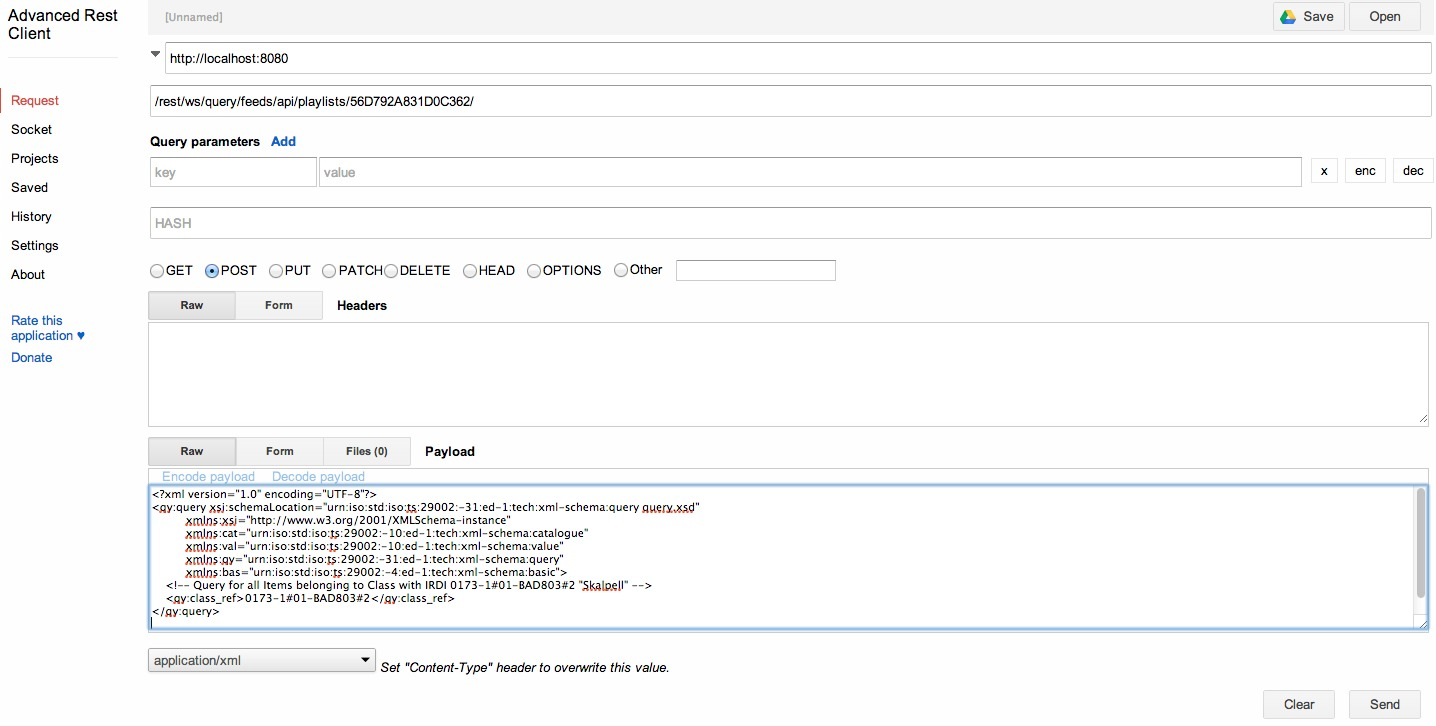
\includegraphics[width=0.98\textwidth]{images/advanced_rest_client_test.jpg}
	\caption{Advanced REST Client Test des Webservices}
	\label{fig:advancedrestclienttest}
\end{figure}

